\chapter{Background}
\label{chap:background}



\section{Coloured Petri Nets}
Common usage: Process and protocol modeling, concurrent programming. Operations:
Simulation, verification and analysis. More recently also software design.

Short intro to places, transitions and arcs?

\section{CPN Tools}

Graphical tool used to design CPN models. 

Reference, with url

\subsection{Standard ML}

Functional language. (Ref) We will call it SML.
Give examples

\subsection{Declarations}

\section{WebSocket}

This section is about the WebSocket
protocol \cite{draft-ietf-hybi-thewebsocketprotocol}.

\begin{figure}
\centering
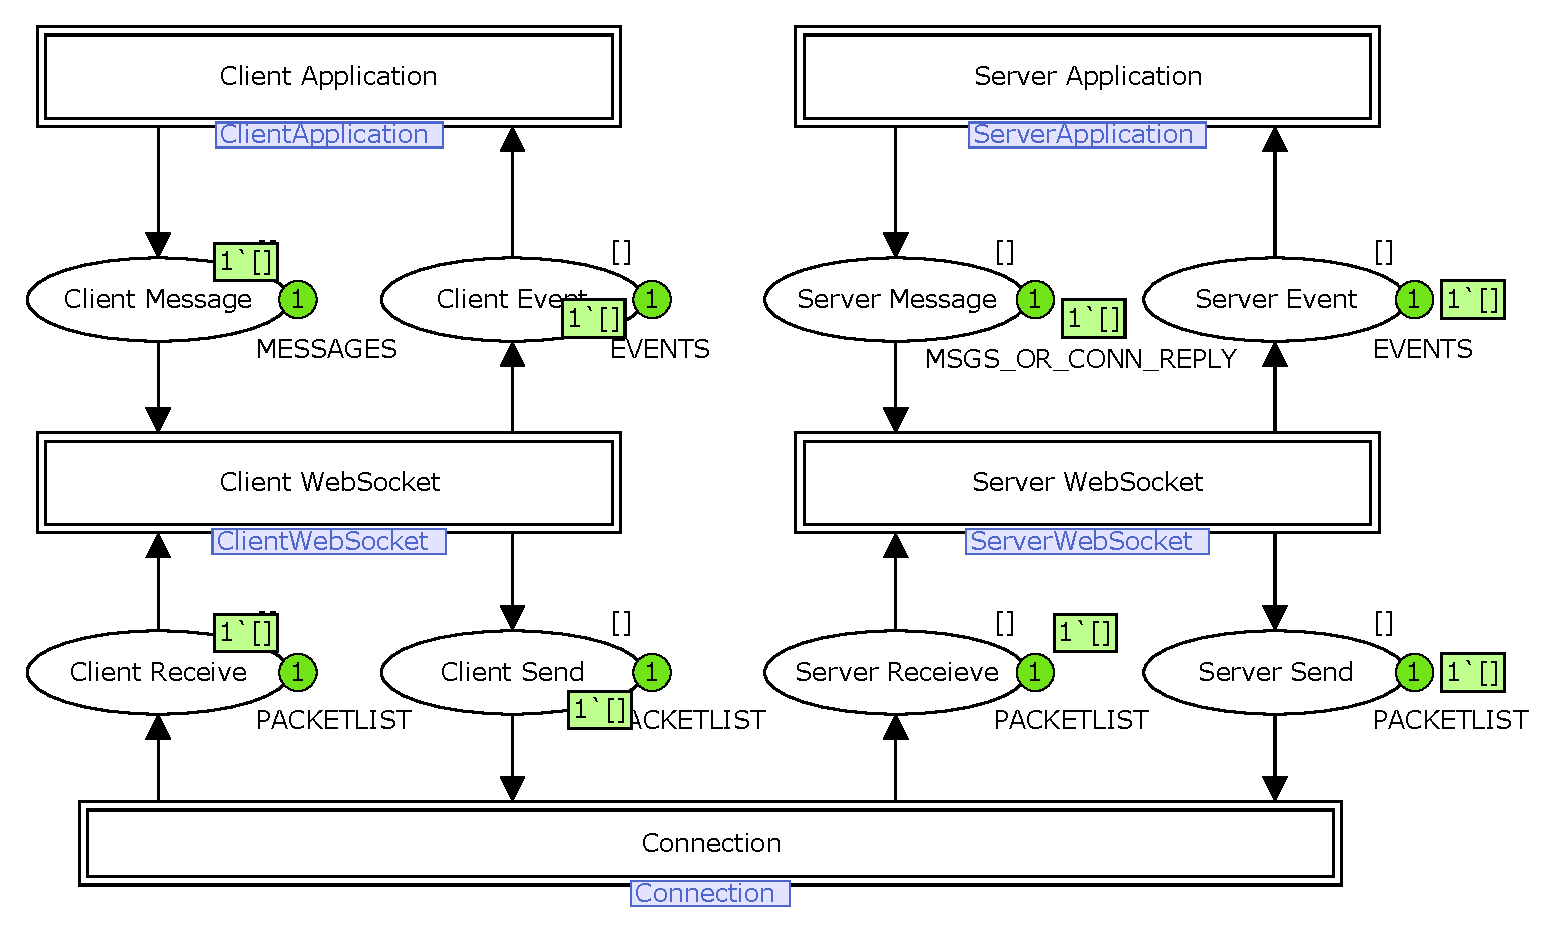
\includegraphics[scale=0.4]{figures/Overview.eps}
\caption{Overview of CPN model of the WebSocket protocol}
\label{fig:overview}
\end{figure}

Shown in Fig.~\ref{fig:overview} is the top-level overview of the WebSocket
protocol as a CPN model. 

Resembles part of OSI model (ref), where top level is levels 6 and 7, middle
level is level 5, and bottom level is levels 4 through 1. Two-way communication
between levels.

Circles represent places. They can contain tokens of a specified colour, and
can have markings to define initial tokens.

Double-bordered represent subpages. These are separate models that have
input and output places that connect to the places on their parent page. We will
examine the first subpage next.

\subsection{Client Application}

\begin{figure}
\centering
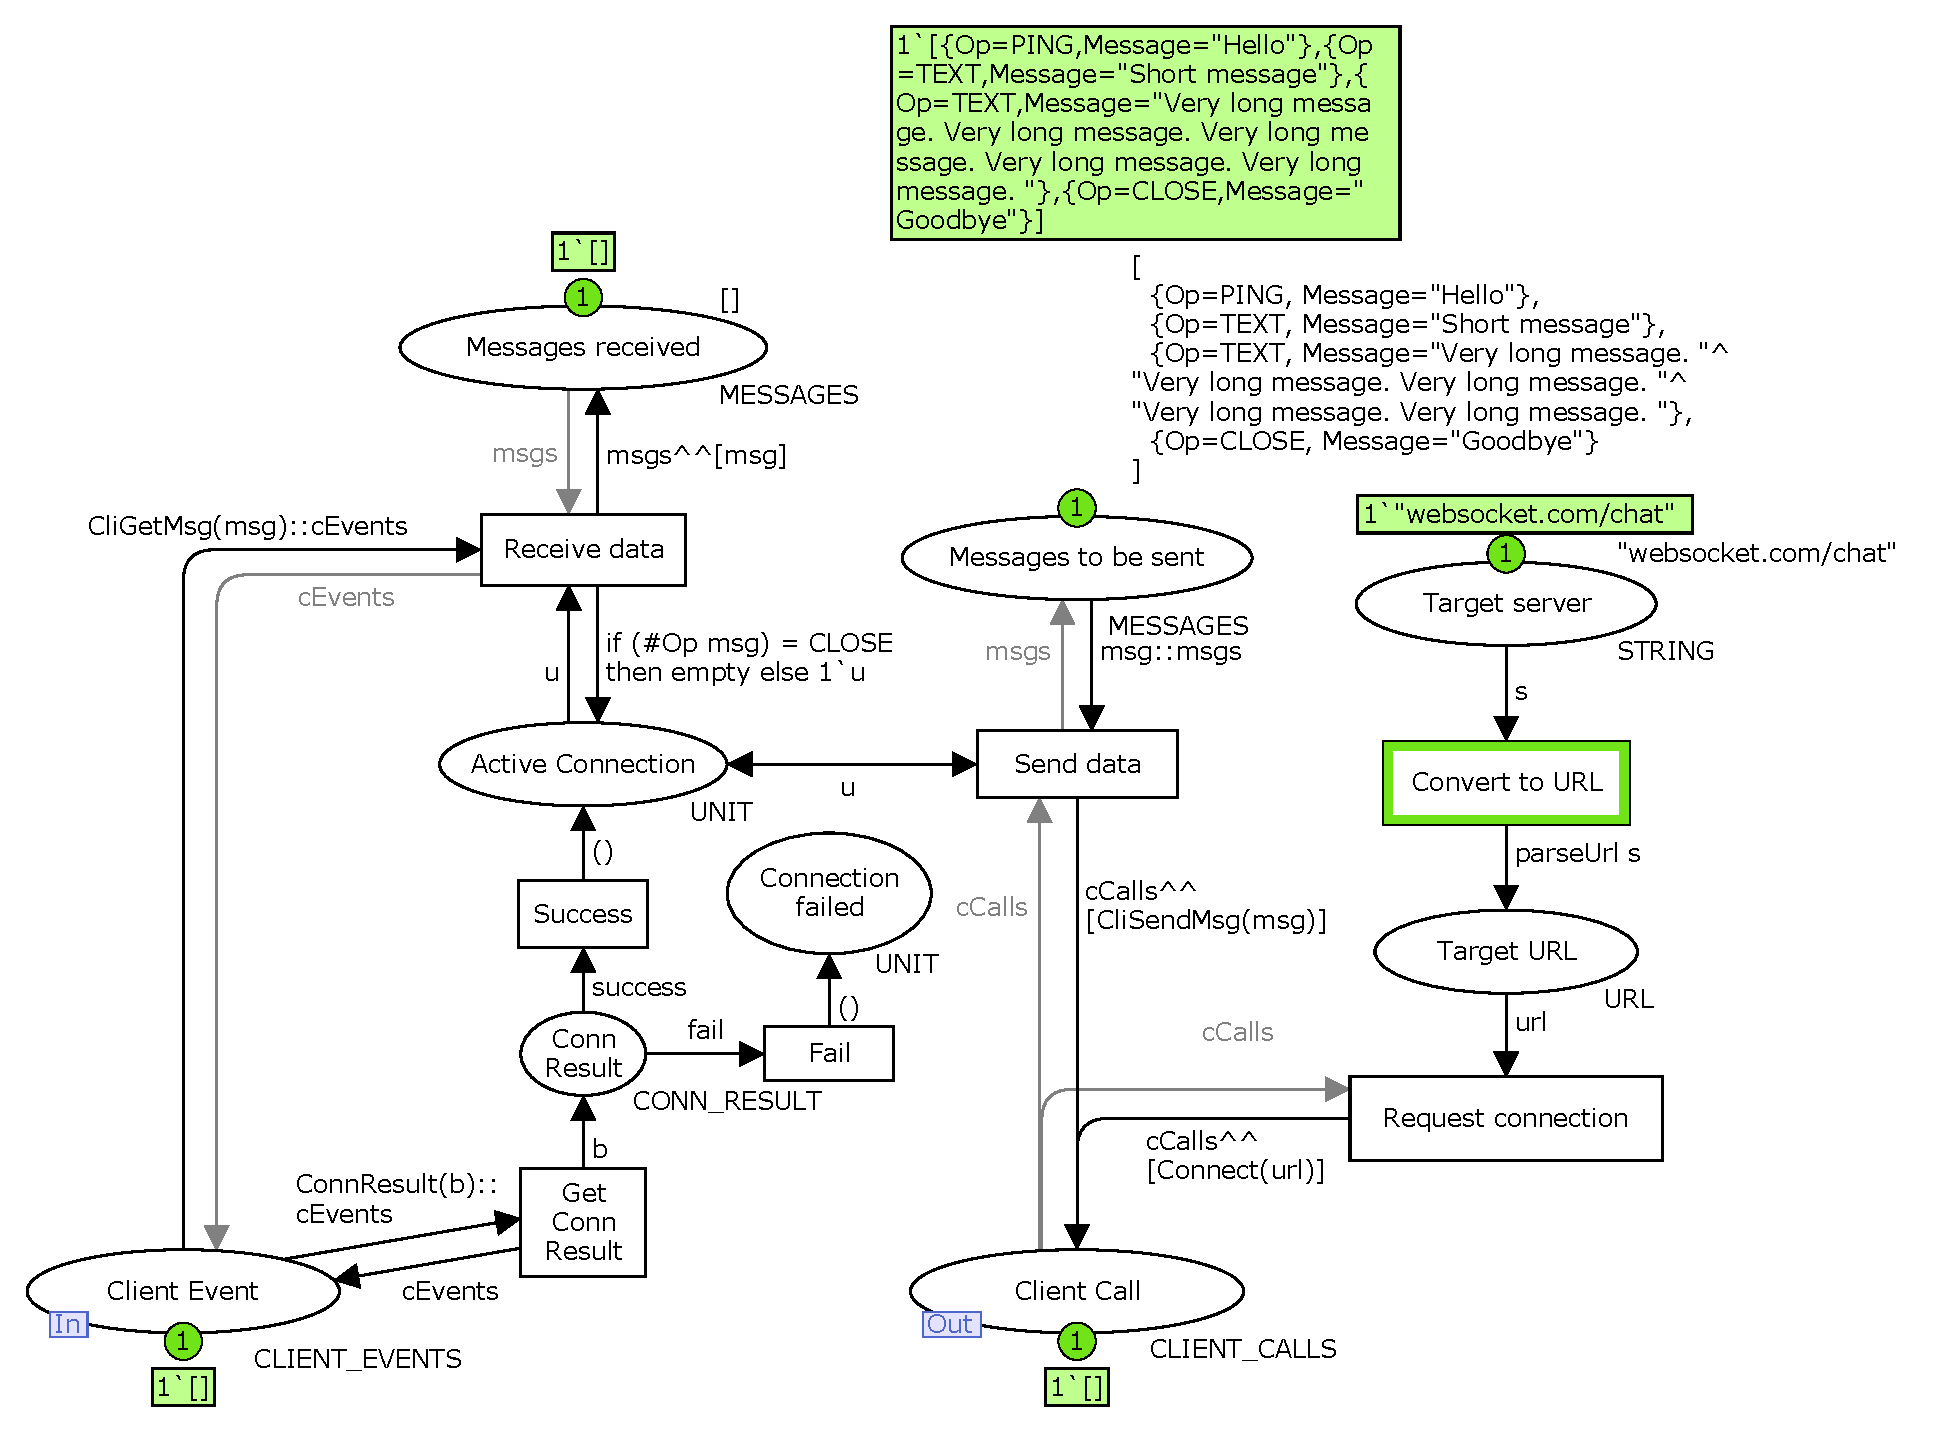
\includegraphics[scale=0.4]{figures/ClientApplication.eps}
\caption{The Client Application}
\label{fig:client_app}
\end{figure}

Laid out from top to bottom to loosely show sequence. 

Bottom places represent interface to WebSocket library. To simplify the overview
model and facilitate easier later expansion, we have only two places that act as
input and output, tagged In and Out. These are connected to the
respective places on the Overview, which are also connected to corresponding places in the
WebSocket Library.

Connect to server
Wait for result
Send and receive data

Here we see an enabled transition at the top. If we were to fire this
transition, it would produce a MESSAGE token in the Send Client Message place.

To the left we see a two-way arc between a place and a transition. This is a
technique used to simulate ordered processing of tokens; queues. We use
lists to do this. To describe a list in SML, we write [] for an empty list and
head::tail for a non-empty list, where head is the first element in the list,
and tail is all the following elements.

So, instead of using the actual color we want in the place, we use a list of
this color. When we want to take an element from the front of the queue,
we use the :: operator to bind the head and tail of the list to variables, and
put only the tail back to the source place. When we want to append an element
to a queue, we concatenate the queue using the \verb|^^| operator with a new
list containing only the new element. To improve readability of the model, these queue operations have
one arc slightly dimmed, to emphasise the flow direction of data.


\subsection{Client WebSocket Library}

\begin{figure}
\centering
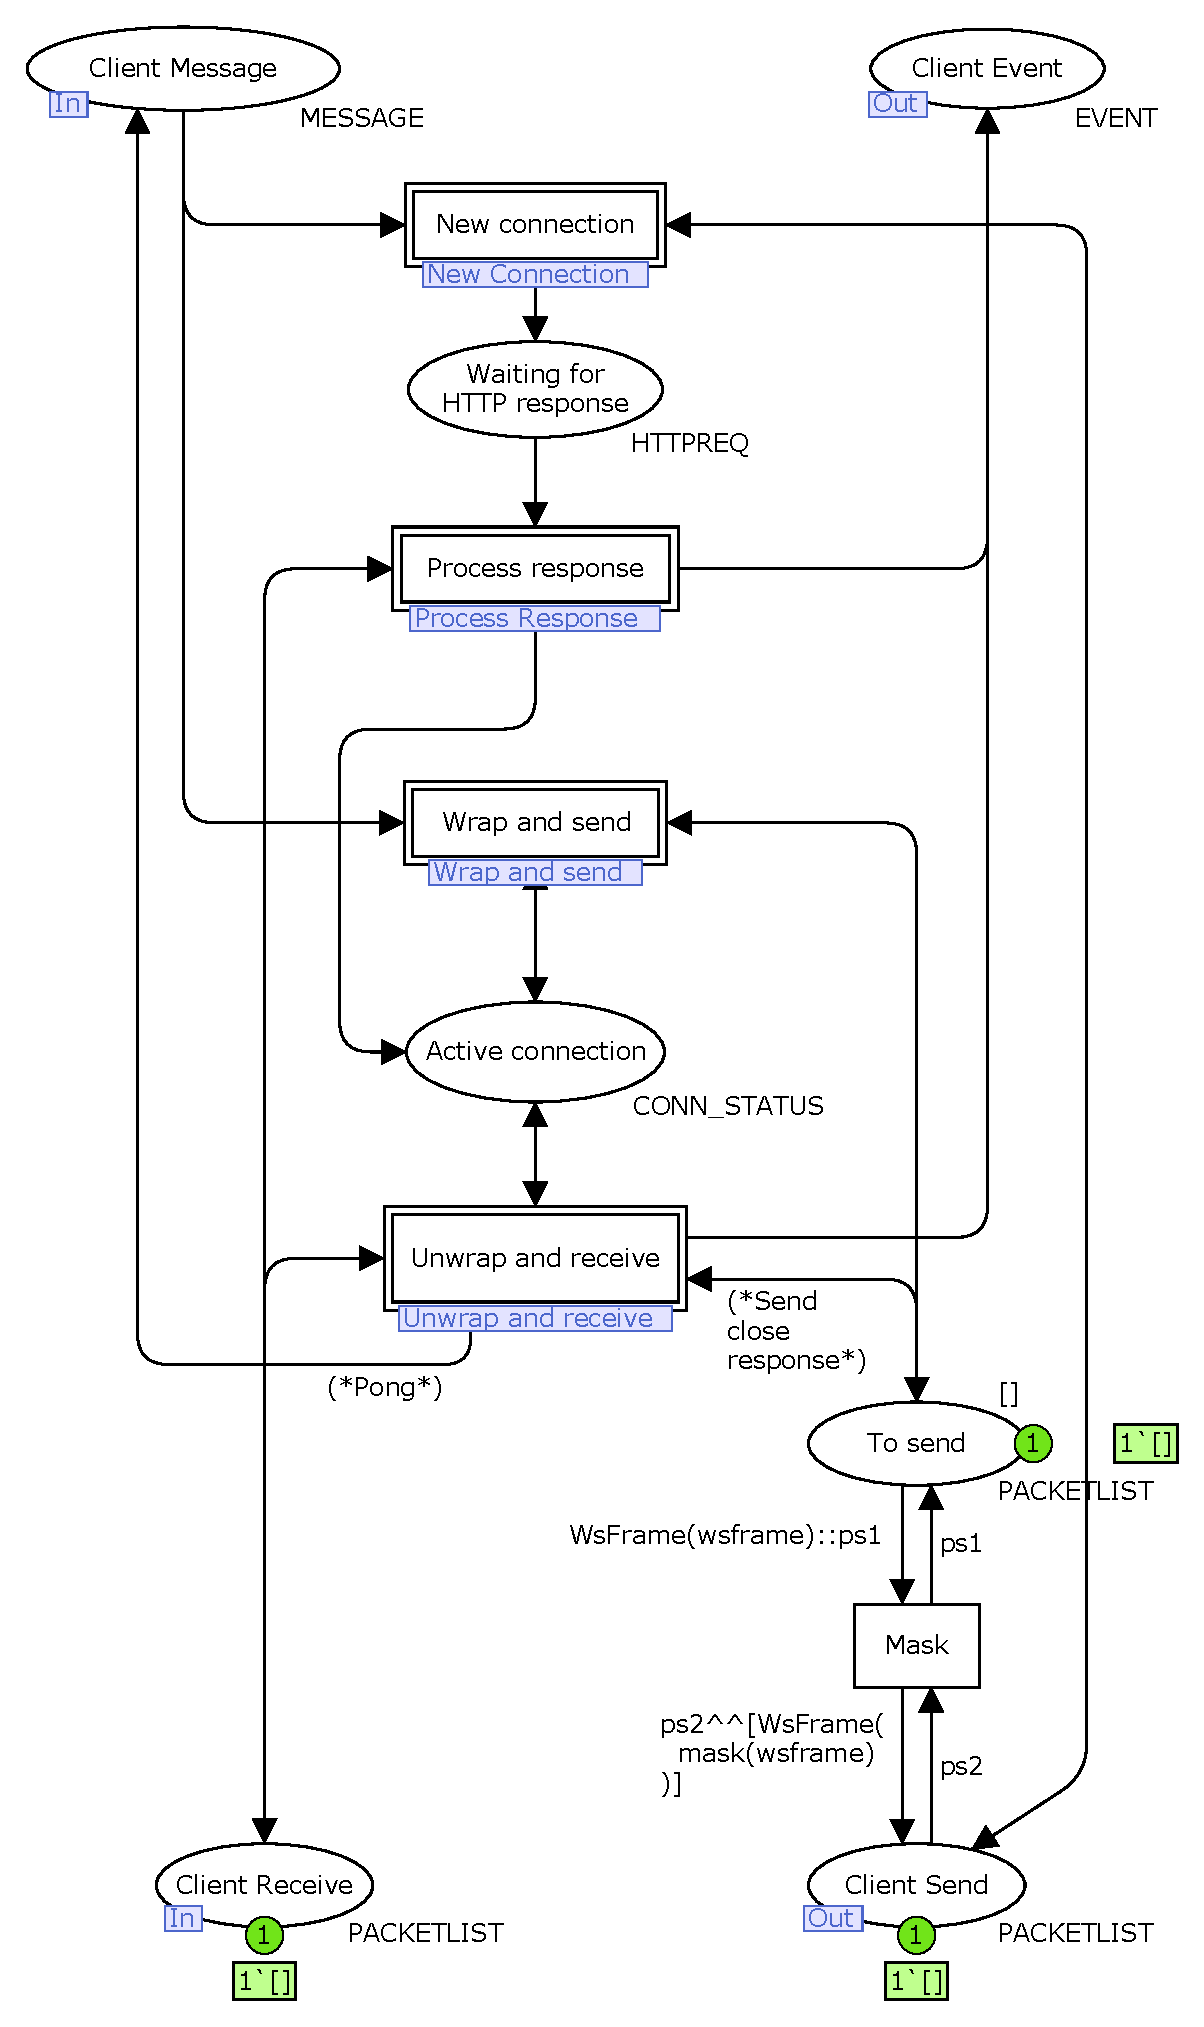
\includegraphics[scale=0.4]{figures/ClientWebSocket.eps}
\caption{The Client WebSocket Library}
\label{fig:client_wslib}
\end{figure}

This page consists mostly of subpages. The only processing being done here is
masking of all websocket frames.

\subsubsection{New connection}


